\documentclass[14pt]{article}
%	options include 12pt or 11pt or 10pt
%	classes include article, report, book, letter, thesis
\usepackage{setspace}
\usepackage{listings}
\usepackage[a4paper, total={6.5in, 9in}]{geometry}
\usepackage{pgfgantt}
\usepackage{afterpage,lscape}
\usepackage{bbm}
\usepackage{amsmath, amsthm, amscd, amsfonts}
\usepackage{graphicx}
\usepackage{pstricks}
\usepackage{natbib}
\setcitestyle{authoryear,open={(},close={)}}
\usepackage{multirow}
\usepackage{tocbibind}
\usepackage{cleveref}
\usepackage{textcomp}
\newtheorem{theorem}{Theorem}
\newtheorem{lemma}{Lemma}
\newtheorem{proposition}{Proposition}
\newtheorem{corollary}{Corollary}
\newtheorem{property}{Property}
\newtheorem{definition}{Definition}
\newtheorem{remark}{Remark}
\usepackage{setspace}
\usepackage[titletoc,title]{appendix}
\usepackage{multirow}
\usepackage{setspace}
\usepackage{epstopdf}
\usepackage{listings}
\usepackage{longtable}
\renewcommand{\baselinestretch}{1.4} 
\usepackage[english]{babel}
\usepackage[utf8]{inputenc}
 
\usepackage{geometry} % to change margins
\usepackage{pdflscape} % provides the landscape environment
\usepackage{ragged2e} % provides \RaggedLeft
 
\usepackage{fancyhdr}
 
\pagestyle{fancy}
\fancyhf{}
\rhead{{\textsf{Vahid Nassiri}}}
\lhead{{\textsf{Final Doctoral Plan: Data Splitting and its Applications}}}
\rfoot{Page \thepage}

\renewcommand{\headrulewidth}{1pt}

 
\begin{document}
\begin{titlepage}


\begin{center}

\includegraphics[scale=1]{KUL.eps}\\
\vspace*{.3cm}
{\sc{\LARGE{Final Doctoral Plan}}}\\
\vspace*{2cm}
{\Huge{\textbf{Data Splitting and its Applications}}}

\vspace*{4cm}
{\LARGE{\textbf{Vahid Nassiri}}}\\
\vspace*{1cm}
{\Large{I-BioStat, KU Leuven}}\\
\vspace*{2cm}
{\Large{Supervisor:}}\\
\vspace*{0.2cm}
{\LARGE{\textbf{Prof. Dr. Geert Molenberghs}}}\\
\vspace*{0.5cm}
{\Large{Co-supervisor:}}\\
\vspace*{0.2cm}
{\LARGE{\textbf{Prof. Dr. Geert Verbeke}}}
\vspace*{2.3cm}


{\Large{April 2017}}

\end{center}

\end{titlepage}
\newpage
{\large{

\textbf{Title}: {\Large{Data Splitting and its Applications}}
\vspace*{0.5cm}

\textbf{Name of applicant}: {\Large{Vahid Nassiri}} (r0292876)
\vspace*{0.5cm}

\textbf{Supervisor}:

{\Large{Prof. Dr. Geert Molenberghs,}} 

I-BioStat, Universiteit Hasselt, Diepenbeek, Belgium.

I-BioStat, KU Leuven, Leuven, Belgium

\vspace*{0.5cm}

\textbf{Co-supervisor:}

{\Large{Prof. Dr. Geert Verbeke,}}

I-BioStat, KU Leuven, Leuven, Belgium,

I-BioStat, Universiteit Hasselt, Diepenbeek, Belgium.

\vspace*{0.5cm}
\textbf{Address}: 

I-BioStat, KU Leuven
Kapucijnenvoer 35 3000 Leuven, Belgium. 

Tel: +32 (0) 16 37 46 96, 

Email: vahid.nassiri@kuleuven.be

\vspace*{0.5cm}
\textbf{Available Grant}: IWT- SBO/ Exascience/ IAP 

\vspace*{0.5cm}
\textbf{Doctoral School Programme}: Patient Related and Public Health Research
\vspace*{0.5cm}

\textbf{Full-time or part-time PhD project}: it is a full-time PhD Project 

\vspace*{0.5cm}
\textbf{Starting date}: 1 May 2014 

\vspace*{0.5cm}
\textbf{Expected end date}: 30 April 2018}}




\newpage


\section{Introduction and problem statement}
\label{sec_intro}
Sample size has always been an issue in statistical analysis. While for many years small sample sizes were a central issue, in recent years, large sample sizes too might confront the statistical analyst with serious problems. When large to huge sample sizes concur with complex models, prohibitive computation times, convergence issues, and the mere impossibility to analyze the data with the preferred inferential technique (e.g., full maximum likelihood) can ensue. 

Furthermore, while in the simplest designs all measurements are independent, many designs lead to hierarchical (a.k.a., clustered, correlated, dependent) data \citep{laird1982,zeger1986,verbeke2009, molenberghs2005}. By cluster here we mean a set of measurements repeatedly collected for one single unit (e.g., subject, household, trial, etc.). Therefore, the number of repetitions refers to the number of measurements available per cluster. Examples include: patients measured repeatedly over time, several patients attending the same general practitioner or clinic, several links clicked by a specific user, genetic data available for a person, etc. Some important examples of clustered data are repeated measurements, longitudinal data, multi-center studies, and meta-analysis. Accounting for such correlations remains a challenge today, when the total number of clusters is large and/or there are a large number of repetitions per cluster. This would sometimes result in prohibitive computations. 

Consider a study which measures (at most) $m$ outcomes for $N$ clusters, each $n_i$ times. Let $y_{rij}$ be the $j$th measurement taken on the $i$th cluster for the $m$th outcome, $i=1,\ldots,N$, $r=1,\ldots,m$ and $j=1,\ldots,n_{ri}$. A general scheme of such data is presented in Figure~\ref{fig_scheme}. As it was mentioned, fitting a model to such data could become challenging when the size of dataset make it eligible for the title \emph{big data}. A dataset could be entitled as \emph{big data} in different situations. In case of the clustered data of interest in this PhD research, data are considered to be big if at least one of the following applies:
\begin{itemize}
\item When the sample size, $N$, becomes very large,
\item When the cluster sizes become very large:
\begin{itemize}
\item When the number of measurements per outcome for some clusters, $n_{ri}$'s, becomes very large,
\item When the number of outcomes, $m$, becomes very large.
\end{itemize}
\end{itemize}
\begin{figure}
\centering
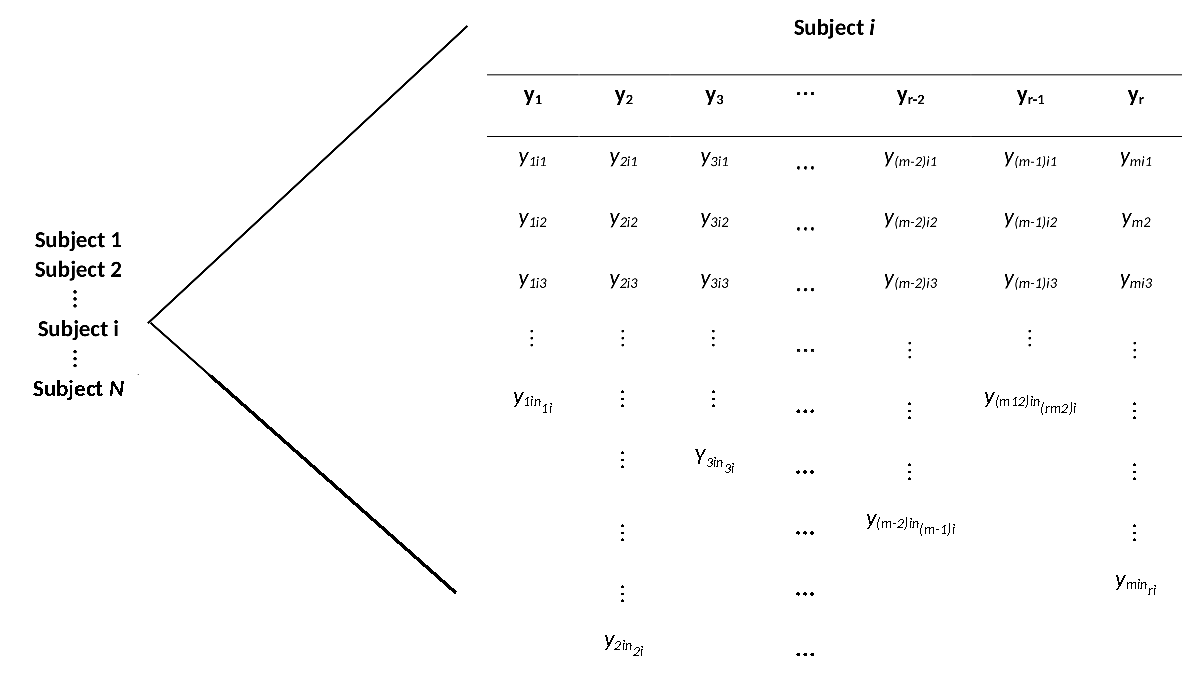
\includegraphics[width=\textwidth]{scheme_new.eps}
\caption{General scheme of the data we consider through this PhD research.} 
\label{fig_scheme}
\end{figure} 
A large sample size could increase the computation time dramatically. On the other hand, even with small sample sizes, having large clusters may increase the computation time. Doing the computations and achieving convergence would become more challenging when the clusters are highly unbalanced (a wide range of cluster sizes). Also, having too many outcomes would increase the number of parameters in the model, to the point at which it could not be feasible any more.  

In this PhD research, such situations are considered and we aim to propose methodologies to deal with such problems using the so-called data splitting. In a nutshell, data splitting means to split the difficult (sometimes infeasible) job of modelling the big data by splitting it into smaller chunks of manageable sub-data, analyze each of them separately, and then combine the results of these analyses using appropriate combinations rules. This would break a difficult task into several, often so-called embarrassingly parallel, simpler tasks.

The rest of this report is structured as follows. In Section~\ref{sec_objective} the main objectives of this PhD research will be briefly reviewed. The datasets motivating our research will be presented in Section~\ref{sec_data_sets}. Section~\ref{sec_idea} describes the general idea behind the methodologies we are developing. The results obtained so far will be presented in Section\ref{sec_results_so_far}. The work in progress as well as a timeline for finishing them will be given in Section~\ref{sec_progress}. Finally, a provisional structure for the upcoming PhD thesis is proposed in Section~\ref{sec_structure}. 

\section{Main objectives}
\label{sec_objective}
Considering the problem stated in Section~\ref{sec_intro}, our main objective is to develop a unified framework that helps researchers to deal with big data in the situations we have described. We expect this framework to have the following properties.

\begin{itemize}
\item The developed framework should be as independent as possible from the modelling approach. In other words, it should be compatible with various modelling approaches, e.g.,  linear, generalized linear, non-linear, etc.
\item As the end-user of this product will be researchers of different fields with different tastes of data analysis systems who are dealing with big data, the developed methodologies should preferably be easy to understand and implement in different platforms, e.g., \textsf{R}, \textsf{SAS}, \textsf{Matlab}, \textsf{Python}, \textsf{Julia}, etc.
\item It goes without saying that a combination of the situations we have described in Section~\ref{sec_intro} could happen for a single set of data. For example, a dataset would consist of a large number of clusters (large $N$), and each of these clusters could be large as well (large $n_{ri}$'s), see Amazon book ratings in Section~\ref{sec_data_sets}. Or large number of outcomes of interest can happen with large number of clusters, see divorce in Flanders dataset in Section~\ref{sec_data_sets}. Therefore, our proposed methodologies for each situation should have the possibility of being combined to deal with a combination of the mentioned situations.
\item This unified approach is going to be implemented in freely available statistical package \textsf{R}. So every interested person can use it without the trouble of implementation. This implementation should be done as efficient as possible.
\item Finally, we should be able to apply our proposed methodology to solve the problems involving our motivating datasets. Considering the diversity of them, that would prove the usefulness of our approach to deal with 21st century real world big data problems.
\end{itemize}




\section{Motivating datasets}
\label{sec_data_sets}
A brief summary of the datasets motivating our research is presented in this section.
\paragraph*{A developmental toxicity study:} This study investigates the dose-response
relationship in mice of the potentially hazardous chemical compound di(2-ethylhexyl)phthalate
(DEHP), used in vacuum pumps and as plasticizers for numerous plastic devices made of polyvinyl chloride. The developmental toxicity study, conducted in timed-pregnant
mice during the period of major organogenesis has attracted
much interest in the toxicity of DEHP. The doses selected for the study were 0, 0.025, 0.05, 0.1,
and 0.15\%, corresponding to a DEHP consumption of 0, 44, 91, 191, and 292 mg/kg/day, respectively.
The dams were sacrificed, slightly prior to normal delivery, and the status of uterine implantation sites recorded. A total of 1082 live fetuses were dissected from the uterus, anesthetized, and examined for external, visceral, and skeletal malformations, as well as for body
weight. Our focus will be on the continuous weight outcome. Evidently, fetuses are clustered within mothers; hence the implied association needs to be accommodated in the analysis. As each mother has different number of fetuses, we have clusters of different sizes. 


\paragraph*{Divorce in Flanders:} This dataset is collected at Centre for Sociological Research, KU Leuven. The data concerned on studying and comparing the personality among
three generations in about 4000 Flemish families. Each family would at most consist of mother, father, step-mother, step-father, one child, grand mother, and grand-father. The personality is measured using the so-called
Big Five Inventory (BFI) score. These scores are built upon 5 factors which in total are measured through 44 items. The usual factor analysis would lose most of the information in the data. Therefore, an idea is to model different combinations of the 5 aspects of personality for each family role using a mixed model. This means, for each family we will have up to 35 responses. The large size of families would add to the difficulty of the problem.

\paragraph*{Hearing data:} To evaluate the hearing performance of a subject, hearing threshold sound pressure levels (measured in dB) are considered. By definition, a hearing threshold is the lowest signal intensity possible to perceive by a subject at a specific frequency. In a study considered in \cite{verbeke2009} and \cite{Verbeke2006}, hearing threshold measured in 11 different frequencies between 125 Hz and 8000 Hz for left and right ears obtained on 603 male participants from the Baltimore Longitudinal Study of Ageing, BLSA. The number of visits for each subject which varies between 1 to 15 are unequally spaced. Modelling these 22 frequencies together is a challenge for the methodologies we developed in this PhD thesis.

\paragraph{Leuven diabetes project:} In order to study how well diabetes is controlled, three outcomes were measured for each patient at baseline ($T_0$) and one year later ($T_1$). These three outcomes of interest were LDL-cholesterol (low-density lipoprotein cholesterol, mg/dl), HbA1c (glycosylated hemoglobin, \%), and SBP (systolic blood pressure, mmHg). Although these three variables are continuous, the interest was in expert-specified cut-off values of these outcomes. The cut-off values are defined as $\{<100, [100,115), [115, 130),\geq 130 \}$ (mg/dl) for LDL-cholesterol, $\{<7, [7, 8), \geq 8\}\%$ for HbA1c, and $\{ \leq 130, (30,140],(140,160],>160\}$mmHg for SBP. Modelling these 3 ordinal outcomes together provides a suitable platform to study the performance of our proposed methodologies dealing with non-Gaussian data.

\paragraph*{Amazon book ratings:} These data consist of the ratings of the books on the Amazon website which are recently made publicly available. The dataset contains $2,330,066$ books, which are rated at least $1$ and at most $21,398$ times. This is an example of clustered data with large highly unbalanced clusters and a large sample size.

\paragraph*{Clinical Trials in Schizophrenia:} These data were collected from five double-blind randomized clinical trials to compare the effects of two treatments for chronic schizophrenia: risperidone and conventional antipsychotic agents. Subjects who received doses of risperidone (4–6 mg/day) or an active control (haloperidol, perphenazine, zuclopenthixol) have been included in the analysis. Patients were clustered within country, and longitudinal measurements were made on each subject over time. The number of patients ranges from 9 to 128 per country with a total of 2039. The
positive and negative syndrome scale (PANSS) was used to asses the global condition of a patient. This scale is constructed from 30 items, each taking values between 1 and 7, giving an overall range of 30 to 210. PANSS provides an operationalized, drug-sensitive instrument, which is useful for both typological and dimensional assessment of schizophrenia. Depending on the trial, treatment was administered for a duration of 48 weeks with at most 12 monthly measurements. Because not all subjects received treatment at the same time points and, not the same amount, the final dataset is unbalanced. Our analysis shows AR(1) structure could be a good candidate for modelling the covariance matrix of the random effects, which is useful to illustrate some of the methodologies we have developed.



\paragraph*{Age-related macular degeneration (ARMD):} The data come from a clinical trial in age-related macular degeneration (ARMD), which is a disease of the retina that causes severe central vision loss. The data consist of a multi-center study (17 centers) to evaluate the effect of an experimental treatment based on interferon-$\alpha$ in a group of patients who were randomly allocated to either placebo or interferon-$\alpha$. The outcome of interest was the change in visual acuity over time. Using standard vision charts, the visual acuity was measured by the number of letters that were correctly read by the patient. The data is used in the context of surrogate endpoint evaluation. The goal of this analyses is to examine if  visual acuity at week 24 could be an appropriate surrogate for the one at week 52, the so-called true endpoint. To this end, the surrogate and the true endpoint have to be modelled jointly. Because of the bivariate nature of the model, coupled with the multi-centre nature of the study, a mixed model is used, by which surrogate evaluation measures are estimated. The data however is highly unbalanced and only has 17 clusters. This makes the iterative algorithms to face with difficulty in convergence. We try to use the methodologies developed in this PhD research to deal with this problem.

\paragraph*{Leuven eyes study:} This is an extensive observational study of glaucoma performed at the ophthalmology department of KU Leuven. The dataset so far consists of 141 variables measured in 614 subjects. As measuring all of these variables was not possible for all of the subjects, this dataset exhibits considerable missingness. Considering the size of dataset and amount of missing values, applying multiple imputations and determining the number of imputations is challenging in this change. 

\section{Data splitting: the general idea}
\label{sec_idea}
As it was briefly mentioned in Section~\ref{sec_intro}, the data splitting approach consists of 3 steps:
\begin{enumerate}
\item Splitting the data.
\item Performing the analysis on each sub-data.
\item Efficiently combine the results from each sub-data to form an overall estimate with its precision.
\end{enumerate}
Let us briefly go over our approaches to deal with each of these steps. 

The first step of this procedure is determined by type of the big data we are dealing with. We divide the data splitting methods based on two main characteristics: 1- independent or dependent sub-samples, 2- random or structured sub-sampling.

Data splitting can be done horizontally or vertically. If the splitting is done at the subject level (each subject will be fully presented in sub-samples), it is called horizontal splitting. The reason of using such a terminology can be observed in Figure~\ref{fig_scheme} (left). Splitting at the subject level means splitting the full data into smaller pieces using horizontal slices. Considering the assumption of having independent clusters, this will result in independent sub-samples. Unless the sub-samples are overlapped, i.e., one subject appears in more than one sub-sample\footnote{Note that, while perfectly possible, the overlapped horizontal splitted sub-samples are not considered in this thesis. One can look in vast literature of bootstrap methods for such an approach.}.

On the other hand, when splitting is done within each subject (part of the measurements for each subject are presented in each sub-sample), it is called vertical splitting. The right-side of Figure~\ref{fig_scheme} shows the reason behind this title. Splitting the measurements within the subject means to take the sub-samples vertically. Such sub-samples will be dependent, since they are measured for a common subject.

Each of horizontal or vertical splitting can be done at random or based on a pre-specified structure.  Here we briefly describe the four different combinations of vertical/horizontal and random/structured data splitting.

\begin{itemize}
\item \textbf{Random horizontal data splitting.} This approach is useful when the number of clusters is large, and preferably the clusters are roughly of equal size, i.e., an (almost) balanced design. This will produce several sub-data with smaller sample sizes which are easier to handle.
\item \textbf{Structured horizontal data splitting.} This approach is useful when some specific clusters are more convenient to deal with when they are together. Therefore, instead of taking random sub-samples, the sub-sampling can be done based on this pre-specified structure. An important example of this approach which is considered in this PhD research is splitting based on the cluster sizes, i.e., forming sub-samples consist of clusters of equal size. This would lead to balanced sub-samples. We have shown existing of closed-form solutions, as well as, faster convergence can be achieved using this approach.
\item \textbf{Random vertical data splitting.} This approach is useful when we are dealing with data with large number of measurements for each cluster per outcome (large $n_{ri}$'s). In this situation one can take sub-samples of each cluster with a manageable size $n_{f(ri)} < n_{ri}$. Obviously, this can be done by taking overlapping (sub-sampling with replacement) or non-overlapping (sub-sampling without replacement) sub-samples.
\item \textbf{Structured vertical data splitting.} This approach is useful when the number of outcomes of interest, $m$, is large. While fitting a model to $m$ outcomes could become heavy or infeasible, fitting models to all possible pairs (triples, etc.) of these outcomes is feasible. That means each sub-sample should consist of all of the measurements for each subject regarding the pair of interest. Therefore, the sub-samples are taken using a pre-specified structure.
\end{itemize}
Obviously, according to type of big data one is dealing with, all of the the combinations of random/structured and horizontal/vertical data splitting can be freely combined. The combination rules then should be combined accordingly. This enables the proposed framework to deal with a combination of the big data situations described in Section~\ref{sec_intro}.


After splitting the data into appropriate sub-samples, the next step is to perform the necessary analysis on these sub-samples. The analysis performed on each sub-sample does not need to be similar to one another. For example, consider 3 outcomes of interest of types continuous, binary, and ordinal. If sub-samples are taken using a structured vertical splitting approach, and each sub-sample consists of pairs of outcomes, the model fitted to each sub-sample will depend on the type of the responses presenting there. Furthermore, the explanatory variables of the models within each sub-sample does not need to be identical across sub-samples. Therefore, such a framework is compatible with different modelling approaches.

The last step of this procedure is combining the results obtained from various sub-samples. As the models fitted within each sub-sample have some common parameters, each parameter of the initial model could possibly be estimated more than once after the second step. We propose to use a weighted average of them to obtain a unique estimation for each parameter. The critical part is to define such appropriate weights. They have to be computed proportionally to the number of clusters within each sub-sample. Also, if needed, size of these clusters should be involved. We have also computed optimal combination weights in order to minimize the final combined variance.

Computing the precision of such an estimator is another important aspect. Computing this precision depends on whether the sub-samples are dependent or independent. For independent sub-samples, one can simply use an average of the obtained variances from each sub-sample. For dependent sub-samples, this averaged variance should be corrected for the information the overlapped sub-samples share. This correction is done using a sandwich estimator \citep{Verbeke2006, Verbeke2007} and multiple ouputation \citep{hoffman2001, follmann2003}.


\section{Results obtained so far}
\label{sec_results_so_far}
We present the results obtained so far through the published, accepted, and submitted papers. The working papers and projects will be presented in Section~\ref{sec_progress}.


\begin{itemize}
\item[--]{\textsf{Lisa Hermans, Vahid Nassiri, Geert Molenberghs, Michael G. Kenward, Wim Van der Elst, Marc Aerts, and Geert Verbeke}}, {\it Clusters with random size: maximum likelihood versus weighted estimation}, Submitted to Statistica Sinica.
\end{itemize}
This paper considers the case of structured horizontal splitting for a dataset consists of vectors of random variables with multivariate Gaussian distribution with compound-symmetry (CS) covariance structure of different sizes. The CS covariance structure considers a common variance for all of the components in the random vector. Furthermore, it assumes all pairs of variables are equally correlated (a common correlation coefficient). We have proposed to split the large sample into sub-samples formed by all clusters of equal sizes. Closed-form solutions are obtained to find the parameter estimates within each balanced sub-sample. The appropriate weights are obtained to efficiently combine estimates from different sub-samples. The closed-form estimates and efficient combination weights are also implemented in \textsf{R}. Simulation results show the derived closed-forms reduce the computation time up to 30,000 times comparing with iterative procedures in \textsf{Proc MIXED} in \textsf{SAS}.



\begin{itemize}
\item[--]{\textsf{Lisa Hermans, Vahid Nassiri, Geert Molenberghs, Michael G. Kenward, Wim Van der Elst, Marc Aerts, and Geert Verbeke}}, {\it Fast, Closed-form, and Efficient Estimators for Hierarchical Models with AR(1) Covariance and Unequal Cluster Sizes}, Communications in Statistics - Simulation and Computation, 2017, DOI: 10.1080/03610918.2017.1316395.
\end{itemize}
This paper considers the same problem as in the previous one, except here the covariance structure is assumed to be autoregressive of order 1, AR(1). In this structure, unlike the CS, the correlation between pairs of variables depends on their distance, i.e., the correlation between $i$th and $j$th components is defined as $\sigma^2 \rho^{|i-j|}$ ($\sigma^2>0$, $-1\leq\rho\leq +1$). The closed-form, fast and efficient estimates are obtained for balanced data following Gaussian distribution with AR(1) structured covariance matrix. The appropriate weights are computed to efficiently combine these estimates and their variances. These closed-form estimates and efficient combination weights are also implemented in \textsf{R}. Simulation results show using the derived closed-forms, the computation time reduced up to 700 times comparing with iterative procedures in \textsf{Proc MIXED} in \textsf{SAS}.



\begin{itemize}
\item[--]{\textsf{Vahid Nassiri, Anna Ivanova, Geert Molenberghs, and Geert Verbeke}}, {\it Fast precision estimation in high-dimensional multivariate joint models}, To appear in Biometrical Journal.
\end{itemize}
In this paper the case of structured vertical splitting is considered when the number of outcomes of interest becomes large. We have proposed to take sub-samples formed by pairs (if needed triples, etc.) of the outcomes. Efficient combination rules were obtained and evaluated using simulations for linear and generalized linear models. The proposed methodology was also implemented in \textsf{R}. Simulation results shows up to 2500 times faster computations comparing with existing procedures.



\begin{itemize}
\item[--]{\textsf{Vahid Nassiri, Geert Molenberghs, and Geert Verbeke}}, {\it Finite information limit variance-covariance structures: Is the entire dataset needed for analysis?}, In High Performance Computing \& Simulation (HPCS), 2016 International Conference on (pp. 736-742). IEEE.
\end{itemize}
We have introduced the concept of a finite information limit (FIL) estimator in this paper. This concerns the situation that amount of information within each cluster is finite. Therefore, after some point adding new observations would not substantially improve efficiency. This means, in case of FIL estimators, one only needs to analyze a small fraction of data to obtain results as efficient as analyzing the full dataset. This concept is introduced in this paper, and some procedures are proposed to detect this property as well as determining the size of this fraction. Comparing with fitting the model to the full data, simulation results show about 1500 times faster computations using this idea.


\begin{itemize}
\item[--]{\textsf{Vahid Nassiri, Geert Molenberghs, and Geert Verbeke}}, {\it A simple, principled rule to determine the number of multiple imputations}, Submitted to The American Statistician.
\end{itemize}
We have discussed the need to take several sub-samples of the original data to deal with big data. In case that these sub-samples are taken with replacement, infinite number of sub-samples can be taken. Furthermore, for sub-sampling without replacement, it is very well possible that taking all possible sub-samples needs enormous amount of time. Thus, the need to use only a part of these sub-samples would emerge. This paper considers the problem of determining the number of sub-samples. Of course, as this problem is similar to the problem of determining the number of imputations when dealing with missing data using multiple imputations, the paper was written with that topic as a target. But the idea is general and can be applied in many situations. It has been used in the FIL paper, and will be used in the IMO paper (see Section~\ref{sec_progress}).



\begin{itemize}
\item[--]{\textsf{Vahid Nassiri, Anik\'{o} Lovik, Geert Molenberghs, and Geert Verbeke}}, {\it On using multiple imputation for factor analysis of incomplete data}, Submitted to Behavior Research Methods.
\end{itemize}
When it comes to factor analysis, principal component analysis, or other methodologies dealing with  eigendecomposition of the covariance matrix, analyzing several datasets in place of the original one would cause some problems at the combination step (Step 3 in our proposed procedure). The reason lies in the fact that not all of the obtained factor loadings would follow the same order. In other words, there is no guarantee that the eigenvector corresponding to the largest eigenvalue of one of these sets of data is comparable with another. This could happen when missing data are multiply imputed, when sub-samples of clusters are taken to overcome computation issues with larger clusters, or when a multilevel factor analysis is of interest, but only at within cluster level. This paper considers this problem and proposed to first estimate the covariance matrix and then perform the factor analysis on the single estimated covariance matrix. The consequences of such an approach are discussed and some criteria are proposed to decide whether this is an appropriate solution or not.



\section{Work in progress}
\label{sec_progress}

We now give an overview of work in progress.

\begin{itemize}
\item[--]{\textsf{Vahid Nassiri, Geert Molenberghs, and Geert Verbeke}}, {\it Iterative multiple outputation: a simple procedure to deal with large clustered data}, In progress.
\end{itemize}
Inspired by finite information limit estimators, we are trying to extend this idea to cases where this property does not hold, or the size of the one sub-sample needed to achieve it is large comparing with available computation power. In this situation, we would suggest to take several smaller random sub-samples. That would involve appropriate rules to determine the number of sub-samples, as well as, combining the results after fitting the models to such sub-samples. Some simulations are already performed, also \textsf{R} functions are written to efficiently take the sub-samples and combine the results of analyses performed on them. Works are on going to apply this methodology on some of our motivating data. The paper would hopefully be submitted before beginning of next academic year.

\begin{itemize}
\item[--]{\textsf{Vahid Nassiri, Anik\'{o} Lovik, Geert Molenberghs, and Geert Verbeke}}, {\it A simple multilevel factor analysis}, In progress.
\end{itemize}
The use of the sub-sampling from different clusters is not restricted to big data. This can also be useful in situations where the intra-cluster correlation is nuisance. Consider the divorce in Flanders data in Section~\ref{sec_data_sets}. There, the main interest, at validation stage, is to verify the BFI structure among the 44 items of the questionnaire removing the correlation imposed by the fact that some of the participants are coming from the same family. This paper considers this problem and try to propose a solutions based on random vertical splitting. The manuscript is in its final levels and we expect it to be submitted within this academic year.


\begin{itemize}
\item[--]{\textsf{Vahid Nassiri, Alvaro Florez Poveda, Luis Adrian Quintero Sarmiento, Wim Van der Elst, Geert Molenberghs, and Geert Verbeke}}, {\it Comparing different approaches for mixed-effects modelling of unbalanced clustered data}, In progress.
\end{itemize}
Although the methodologies we proposed and developed in this thesis are targeting big data, sometimes very small data and very large data suffer from the same issues. One common problem of large and small data is the convergence issues. In this article we try to study the performance of our proposed method to deal with small highly unbalanced data and compare it with other solutions developed in I-BioStat.


\begin{itemize}
\item[--]{\textsf{Vahid Nassiri, Geert Molenberghs, and Geert Verbeke}}, {\it Data splitting: an \textsf{R} package to analyze big clustered data.}, In progress.
\end{itemize}
As mentioned before, for many of the proposed and developed methods \textsf{R} functions have been prepared to make the implementation easier for the end-user. We are planning to make generic functions out of them and collect them in the form an \textsf{R} package which will be publicly available. This will need more time and effort, but we hope it can be accomplished by the end of the PhD.

The last final step in the last year of this PhD research will be preparing the final manuscript of the PhD thesis. Figure~\ref{fig_gant} shows a Gantt chart of the fourth year PhD in order to complete the mentioned tasks.


\begin{figure}
\centering
\begin{ganttchart}[vgrid={draw=none,draw=none},%
             %today=15,%
             %today offset=.5,%
             %today label=Heute,%
             %progress=today,%
             x unit=0.7cm,
             y unit title=1cm,
             y unit chart=0.5cm,
             bar incomplete/.append style={fill=red},%
             progress label text=  {\quad\pgfmathprintnumber[precision=0,verbatim]{#1}\%},
             milestone label font=\tiny,
             group label font=\tiny,
             title label font=\tiny,
             bar label node/.style={text width=5cm,align=right,font=\scriptsize\RaggedLeft,anchor=east},
             milestone label node/.style={text width=3cm,align=right,font=\scriptsize\RaggedLeft,anchor=east},
             group label node/.style={text width=4cm,align=right,font=\scriptsize\RaggedLeft,anchor=east}
             ]{1}{12}
\gantttitlecalendar*[compress calendar,time slot format=isodate]{2017-05-1}{2018-4-30}{year, month} \\
\gantttitlelist{1,...,12}{1}\\
\ganttgroup{Total Duration}{1}{12} \\
  %%%%%%%%%%%%%%%%%Phase-1
\ganttgroup{Finishing research papers}{1}{6} \\
\ganttbar{Paper 1}{1}{1} \\
\ganttlinkedbar{Paper 2}{2}{3} \ganttnewline
\ganttlinkedbar{Paper 3}{4}{6} \ganttnewline

%%%%%%%%%%%%%%%%%Phase-2
\ganttgroup{Preparing the \textsf{R} package}{4}{9} \\
  %%%%%%%%%%%%%%%%%Phase-3
\ganttgroup{Writing the thesis manuscript}{9}{12} \\
%%%%%%%%%%%%%%%%%%%%%%%%%%%%%%%%%%%%%%%%%%%%%%%%%%%%%%%%%%%%%%%
\end{ganttchart}
\label{fig_gant}
\caption{Gantt chart of the provisional fourth year PhD plan}
\end{figure}


\section{Provisional structure of the thesis}
\label{sec_structure}

\begin{itemize}
\item Chapter 1: Introduction and the state of art
\item Chapter 2: Motivating datasets
\item Chapter 3: Problem statement and preliminaries
\item Chapter 4: Horizontal splitting
\item Chapter 5: Vertical splitting
\item Chapter 6: Related topics
\item Chapter 7: Conclusions
\end{itemize}


 

\bibliography{bib_final_plan}{}
\bibliographystyle{abbrvnat}



\end{document}












